\section{Conception — PSM}

\subsection{Choix technologiques}

L'expérience croisée des \emph{BackSynth Boys} nous a conduit à
nous tourner vers le \emph{framework} Qt, dont chacun apprécie
l'API élégante et performante. Ce framework fournit surtout des
outils pour la construction d'interfaces homme-machine, mais il est
très riche et possède également des APIs pour la manipulation de
collections, ou le traitement de documents XML.

La meilleure façon de tirer parti de Qt est de programmer en C++,
c'est donc le langage qui a été choisi pour le développement de
SynthPro.

\subsection{Conséquences sur l'architecture}

\subsubsection{Diagramme de classes de niveau PSM}

\begin{figure}[htb]
\centering
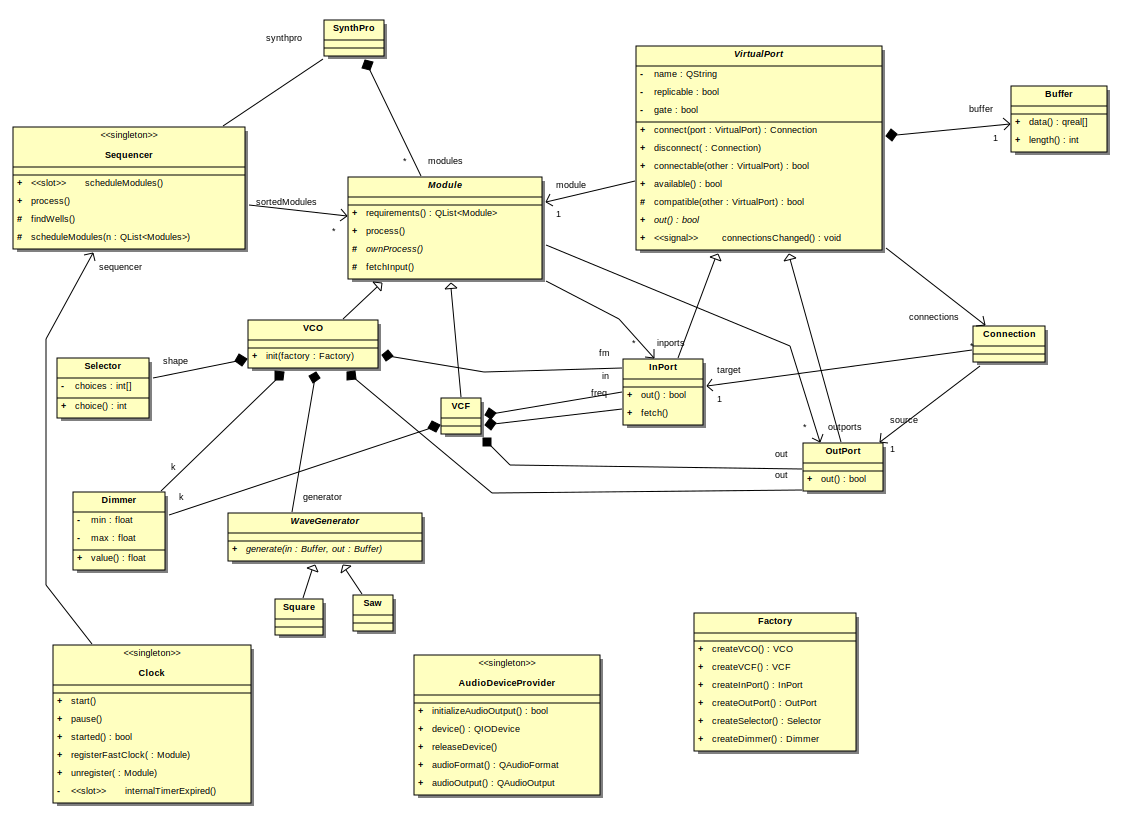
\includegraphics[width=21cm,angle=90]{../img/ps/business-psm.pdf}
\caption{Classes métier au niveau PSM}
\label{psm-class}
\end{figure}

La figure \ref{psm-class} représente les classes métier au niveau PSM. Il n'y a
pas vraiment de changement profond par rapport au niveau PIM, les
types de données de Qt sont utilisés (\verb!QList!, \verb!QString!,
etc.), et des \emph{signals} et \emph{slots} apparaissent. Un
\emph{signal} est une notification qu'un composant émet pour
informer d'un événement, un \emph{slot} est une opération
(\emph{handler}) qui peut être appelée pour gérer cette
notification. Le système de \emph{signals} et \emph{slots} est une
implémentation proposée par Qt du patron de conception
\emph{Observer}.

Par exemple, la classe \verb!VirtualPort! émet le \emph{signal}
\verb!connectionsChanged! à chaque fois qu'une connexion ou une
déconnexion a lieu. Ce signal est intercepté par le \verb!SynthPro!
qui demande au \verb!Sequencer! de recalculer l'ordonnancement de
ses modules.

Enfin, la classe \verb!AudioDeviceProvider! fait son apparition,
elle gère l'accès à la carte son en utilisant l'API QtMultimedia.

\subsubsection{Héritage en diamant}

\begin{figure}[htb]
\centering
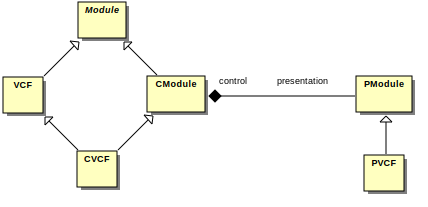
\includegraphics[width=12cm]{../img/ps/pacmodule-psm.pdf}
\caption{Héritage en diamant sur le contrôle du module VCF}
\end{figure}

Notre choix de faire hériter les contrôles des composants de leur
abstraction a conduit à un problème d'héritage en diamant. Nous
avons donc pu goûter aux joies de l'héritage virtuel en C++.

\subsection{Conséquences sur l'interface utilisateur}

Nous avons utilisé le \emph{framework} GraphicsView de Qt pour
gérer l'affichage des modules. Ce \emph{framework} est conçu pour
afficher des objets 2D dans une scène très efficacement.


\subsection{Données, mesures et ordre de grandeur}

\subsubsection{Type des données}

Afin de garder un maximum de précision lors du traitement des
données, nous avons choisi d'utiliser des \verb!double!. Une autre
alternative aurait été d'utiliser des entiers, mais cela ne
correspondait pas aux ordres de grandeur que nous souhaitions
représenter (voir section suivante), à moins de normaliser et
dénormaliser nos signaux selon le traitement, source de plus de
complexité et peut-être même de pertes de performances.

\subsubsection{Signaux entre les modules}

Nos modules étant supposés simuler du matériel analogique
manipulant des tensions, nous avons généré et traité des signaux de
même dimension. Ainsi, un VCO produira un signal allant de -5V à
+5V et une sortie Gate Out de 0V à 1V. De même, notre note musicale
de référence est un DO de l'octave 4, correspondant à 0V. Une
octave représente 1V, donc un DO--5 correspond à 1V, et un DO-3 à
-1V.

\subsubsection{Signaux pour la carte son.}

La sortie son utilisant du 16 bits, nous normalisons le signal au
maximum de ce que la carte son peut supporter, soit de -32767 à
32767.

\subsubsection{Gestion du débordement}

Notre logiciel simulant du matériel, mais pas leur comportement
électronique exact, il nous est tout à fait possible de générer des
tensions que les synthétiseurs seraient (heureusement !) incapables
de produire. Pour éviter tout débordement, chaque sortie (qu'elle
soit audio ou non) dispose d'un test aux limites afin de saturer
plutôt que de déborder. De plus, chaque VCO dispose lui aussi d'un
limiteur en sortie, évitant le débordement des opérations
arithmétiques, notamment si les modules sont mis en boucle.

